\subsection{Time Delay}
    $y(t) = e^{s(t-T)} = e^{-sT} u(t) \rightarrow$ Time delay is given by $e^{-sT} \overset{\text{Padé}}{\approx} \frac{\frac{2}{T} - s}{\frac{2}{T} + s}$ (Useful for Root Locus)\\
    Magnitude plot stays the same, angle goes to $-\infty$ for increasing $\omega$ (Phase is shifted back by $\omega T$)\\
    Time delay can make the plot make encircle the $-\frac{1}{k}$ Point
    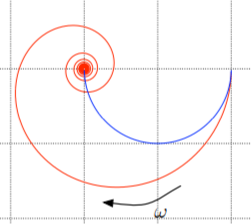
\includegraphics[width = \linewidth]{src/images/time_delay_nyquist.png}
    Relation of phase margin with ($\phi_{\text{m, T}}$) and without ($\phi_{\text{m, T}}$) time delay and crossover frequency ($\omega_c$):
    \begin{align*}
        \phi_{\text{m, T}} = \phi_{\text{m, 0}} - \omega_c T
    \end{align*}
    Design system ignoring time delay, check PM using relation above, add Lead- / Lag-controller, increase gain